
\chapter{Dialogové systémy}\label{chapter-theory}

Toto je teoretický úvod představující důležité pojmy.
Jak název napovídá, dialogové systémy vedou dialog s uživatelem. Jsou to
tedy jakékoliv programy (nebo skupiny programů) využívající
pro komunikaci přirozený jazyk, obvykle ve formě textové nebo hlasové.
Vyčerpávající shrnutí tohoto tématu, souvisejících problémů a metod
jejich řešení podávají \citet{jurafsky_slp_2020}. Za zmínku jistě stojí
i kniha \textit{Conversational AI} \citep{mctear_conversational_2020} nebo
článek \textit{Neural Approaches to Conversational AI} \citep{gao_neural_2019},
kde se autoři zabývají aplikací strojového učení.

\section{Dělení systémů}
Dialogové systémy můžeme dělit dle mnoha různých specifik. Asi vůbec
nejzákladnějším je dělení na systémy \textit{zaměřené na plnění úkolů}
(rozšířený je anglický termín \textit{task-oriented}), jejichž úkolem
je dosáhnout nějakého uživatelova cíle; a \uv{\textit{tlachací}} (anglicky
\textit{chitchat}), jejichž úkolem je jen vést s uživatelem smysluplnou
konverzaci \citep[strana 6]{gao_neural_2019}.

\textit{Doménou} systému se rozumí téma, kterému by se měl být schopen
věnovat. Podle toho, zda to dokáže jen u jednoho, nebo u více různých,
můžeme systém nazývat \textit{jednodoménový} nebo \textit{vícedoménový} \citep[strana 47]{gao_neural_2019}.

Dále můžeme systémy dělit podle toho, kdo řídí dialog. Dotaz či změnu tématu
může iniciovat vždy pouze uživatel a systém jen odpovídat, nebo naopak, nebo
se mohou v iniciativě střídat \citep[strany 495-496]{jurafsky_slp_2020}. Implementace posledního jmenovaného je samozřejmě
nejkomplikovanější.

Posledním dělením, které uvedeme, je podle kanálů komunikace, tedy
v jaké prvotní formě je informace mezi uživatelem a systémem předávána.
Obvykle je forma na obou stranách stejná, může se však i lišit. Mezi
nejčastější patří text, mluvená řeč a obraz (ať už statický nebo
dynamický), ale existují již i humanoidní roboti schopni vyjadřovat emoce pomocí
mimiky, jakého popisují \citet{faraj_facially_2021} ve svém článku.

My se nadále budeme zabývat systémem zaměřeným na plnění úkolů v rámci jedné
domény, který má jako vstup i výstup mluvenou řeč, protože do této kategorie
naše implementace spadá.

\section{Problémy ve zpracování dialogu}

Při trochu podrobnějším pohledu na většinu rozhovorů zjistíme, že nejsou
tak jednoduché a přímočaré, jak si je představíme \citep[sekce 24.1]{jurafsky_slp_2020}. To dále ztěžuje
veškeré strojové zpracování. Některé komplikace umíme řešit jen do určité
míry, některé zatím vůbec. Vezměme si například takovýto smyšlený dialog:

\begin{code}
    A: Dal bych si.. hmmm.. majoránku, tedy pardon! Marokánku.
    B: S sebou, nebo..
    A: Vlastně ne! Raději cheesecake.
\end{code}

Jistě si dokážeme představit, že by mohl proběhnout a připadal by nám
relativně normální. S čím se však musejí aktéři vypořádat? Mluvčí A se
nejdříve rozmýšlí a druhý to musí pochopit a počkat. Poté se rozhodne
a něco řekne, mluvčí B to pochopí, ale vzápětí musí své pochopení
poupravit, protože A se jen přeřekl a opravuje se. Když se B konečně
dostane ke slovu, začne mluvit, ale hned musí zase skončit, protože
A mu skáče do řeči s další opravou -- přeje si cheesecake. Pokud by
však B neznal toto anglické slovo (systém naučený rozpoznávat češtinu
by nemusel), v hlučnějším prostředí by pravděpodobně pochytil spíše
něco jako \uv{čistej}. Nejběžnější problémy, se kterými se v tomto
směru potýkáme, rozebereme v následujících třech podsekcích.

\subsection{Začátek a konec promluvy}

Prvním problémem je jak vůbec zjistit, kdy uživatel dialog začal, kdy
skončil svůj \textit{tah} (souvislou promluvu, po které obvykle očekává odpověď),
a kdy skončil celý dialog \citep[strana 494]{jurafsky_slp_2020}.
Jako lidé většinou začátek dialogu jsme schopni rozpoznat tím, že se na
nás druhý podívá či nás osloví. Pohled u stroje s pouze zvukovým vstupem
detekovat schopni nejsme, oslovení dnešní technologie již dokáží. Většinou
definujeme jedno nebo několik slov, které stroj chápe jako začátek dialogu,
tzv. \textit{wake words}. Součást systému detekující tato slova musí být velmi
výpočetně úsporná, protože musí běžet neustále. Dnes jsou obvykle
využívány komponenty využívající hlubokého učení, jako třeba Howl
\citep{tang_howl_2020}.
Běžným způsobem je ale stále zahájení dialogu stiskem tlačítka či něčím
podobným.

Zahájení jsme tedy detekovali, ale jak poznat konec? Za konec tahu je
většinou považována delší pauza, v takovou chvíli systém vyhodnotí odpověď
a začne odpovídat. Problém je, pokud jsme konec tahu detekovali špatně a
v průběhu systémové odpovědi začne uživatel opět mluvit. V lidské konverzaci
se to stává běžně a umíme se s tím jednoduše vypořádat, protože jsme schopni
zároveň mluvit a poslouchat. U strojů to však problém je, běžnou praxí asistentů
je proto začít znovu poslouchat až po ukončení jejich promluvy.

Existují však již i \textit{inkrementální} dialogové systémy, které
vstup zpracovávají průběžně a detekují konec tahu i jinými způsoby.
Možné způsoby (často využívané i člověkem) popisují \citet{turn_taking_taxonomy_2015},
\citet{khouzaimi_turn-taking_2016} pak ve své práci navrhuje
možnou architekturu inkrementálních systémů a způsob jejich učení.

Úplný konec dialogu většinou detekujeme buď explicitně, zvolenými klíčovými
slovy (třeba \uv{konec}) či frázemi (rozloučení); nebo implicitně, pokud
systém splní uživatelův cíl či uživatel již neodpoví.

\subsection{Zpracování zvuku}

Při převodu mluveného slova na text narážíme na problémy spousty nepřesností \citep[sekce 4.1]{glass_challenges_1999}.
Přepis nám ztěžuje okolní hluk, který dokážeme automaticky odfiltrovat jen do určité míry
a obtížně. Navíc pokud dojde k chybě v nějakém slově, můžeme se ji sice snažit
z kontextu nějak zpětně opravit, ale opět je to složitá práce navíc. Člověk
tyto drobné opravy na základě kontextu dělá podvědomě a bravurně.

Dále se potýkáme s různou výslovností různých lidí, přeřeky, opravami
či výplňovými zvuky, kdy se mluvčí rozmýšlí, co chce říct dál. Zvláště
pokud se něco takového vyskytne uprostřed slova, může být obtížné dát
strojově dohromady výsledek promluvy.

\subsection{Očekávané znalosti, domýšlení}

Při běžné komunikaci člověk od druhého očekává určitou míru přehledu o světě
-- minimálně fakta typu že Slunce je na obloze považujeme za samozřejmá.
Předáváním těchto obecných znalostí dialogovým systémům se ve svém článku
zabývají \citet{young_augmenting_2018}.

Také očekáváme, že druhý bude schopen pochopit význam zájmen, odkazů
a obecně věcí nevyjádřených přímo. Více výrazů odkazujících na jednu věc
označujeme \textit{koreference}, podrobnější popis tématu dává
\citet[kapitola 21]{jurafsky_slp_2020}.


\section{Konstrukce dialogových systémů}

Tradiční přístup implementace bychom mohli označit jako postupný. Čítá několik
komponent, kde každá zajišťuje část práce nutné k porozumění uživateli a
zodpovězení jeho prohlášení \citep[sekce 4.1]{gao_neural_2019}. Takovou konstrukci budeme nazývat \textit{pipeline}.
Tento přístup dobře ilustruje, co všechno vlastně
člověk podvědomě při komunikaci dělá. Druhý přístup reprezentují tzv. \textit{end-to-end}
systémy využívající metod strojového učení, které umožňují nahrazení až
několika komponent jedním modelem \citep[sekce 4.6]{gao_neural_2019}. Taková implementace první uvedený v mnohém
předčí, ale v praxi se příliš nevyužívá z důvodu náročnosti na trénovací data.

Již jsme zmínili, že vícekrokové systémy mají několik komponent, které na sebe
navazují, jedna obvykle určitým způsobem využije výstup z předchozí jako svůj
vstup. Nejčastěji se používá rozdělení na šest částí, kterým se podrobněji
budeme věnovat v následujících podsekcích. Jsou to: převod textu na řeč (v podsekci~\ref{stt}),
extrakce významu (\ref{nlu}), udržování stavu (\ref{dst}), rozhodnutí o dalším kroku (\ref{dp}),
vytvoření odpovědi v přirozeném jazyce (\ref{nlg}) a syntéza hlasu (\ref{tts}). První
a poslední u textových systémů odpadají.

\subsection{Převod mluvené řeči na text}\label{stt}

Zkráceně značíme nejčastěji \textit{STT} z anglického \textit{speech-to-text}.
Jak název napovídá, úkolem této komponenty je převést zvukový projev na text.
Dříve byly k tomuto účelu využívány především \textit{skryté
    Markovovy modely (hidden Markov models, HMM)}. Tyto modely se nazývají skryté,
protože jejich vnitřní stavy nemohou být pozorovány, vidíme pouze výstup.
Jsou postaveny na \textit{Markovových řetězcích}, jejichž základním předpokladem
je, že v sekvenci stavů pravděpodobnost příštího závisí jen na stavu aktuálním,
nikoliv žádném předchozím, jak uvádí například \citet[strana 4]{brooks_handbook_2011}.
Jejich výhodou je, že jsou poměrně jednoduché a nenáročné na výpočetní výkon.

Jako v mnoha jiných odvětvích, i zde přišly ke slovu neuronové sítě, které HMM
ve většině směrů překonaly. V dobrých podmínkách jsou schopny provést přepis
téměř bezchybně \citep{zhang_pushing_2020}. Opět však narážíme i na jejich slabé stránky,
totiž vysokou náročnost na množství trénovacích dat a výpočetní výkon.

O obecných problémech typu okolního hluku či různé výslovnosti jsme se
již zmiňovali. Zde ještě dodáme, že komplikací může být i nedostatečná kvalita
nahrávky. Mimo jiné z těchto důvodů výstupem často nebývá jen jedno
slovo či věta, nýbrž několik spolu s \textit{jistotou}, kterou model této
variantě přiřadil.

\subsection{Extrakce významu}\label{nlu}

\subsubsection{Obecný význam}
Nyní když máme textovou reprezentaci výpovědi, budeme se z ní snažit nějak
jednodušeji vyjádřit podstatné části. Této komponentě se obvykle říká
\textit{porozumění jazyku (natural language understanding, NLU)}. V jistém
smyslu je její úkol nejnáročnější, neboť jazyky mají mnoho nejasností,
víceznačností a nuancí obecně. Výstupem této komponenty je často opět
seznam reprezentací s hodnotou, nakolik si je systém tou konkrétní
interpretací jistý \citep[sekce 4.3]{gao_neural_2019}.

K získání oné jednodušší reprezentace můžeme využít \textit{dialogových aktů}
(\textit{DA}) \citep[strana 494]{jurafsky_slp_2020}. Ty pak
často popisujeme například trojicemi \textit{úmysl}--\textit{slot}--\textit{hodnota},
ale používány jsou různé reprezentace. Několik jich popisují a
metodologii pro převod z nich do podmnožiny
ISO standardu navrhují \citet{mezza_iso-standard_2018}.

Použití trojic můžeme ilustrovat na úryvku \uv{v deset hodin}, který bychom
přeložili na trojici
informovat--čas--10:00. K získání relevantních trojic můžeme využít ručně
psané \textit{regulární výrazy} vyhledávající vzorce v textu, tento přístup
je však dost náročný. Pro rozumnou funkcionalitu takových výrazů musíme napsat
stovky. Dnes obvykle lepší alternativou jsou opět modely využívající strojové
učení. Aplikaci hlubokých neuronových sítí na tento problém
popisují \citet{liu_multi-task_2019}.

\subsubsection{Jména a názvy}
Důležitou součástí je \textit{rozpoznání jmenných entit} (anglicky
\textit{named entity recognition, NER}),
kde cílem je rozpoznat v textu názvy, které jako slova sama o sobě nemají
význam, pokud nevíme, že jde o název. Zajímají nás jak jména lidí, tak
geografických objektů či čehokoliv jiného, v závislosti na cílové doméně.

K jejich nalezení se opět často používají modely strojového učení, pro češtinu
jeden takový popsali \citet{ekstein_czech_2019}. Na pomoc či další zpracování
můžeme využít metriky vzdálenosti mezi textovými řetězci,
jako je \textit{Levenshteinova vzdálenost}, pravděpodobně představena autorem v
článku roku 1965 \citep{Levenshtein1965BinaryCC}. Ta říká, kolik nejméně úprav
musíme u jednoho řetězce udělat, abychom dostali druhý, tedy zjednodušeně řečeno
jak moc jsou si dva řetězce podobné. Trochu problém nastává u krátkých slov,
protože u nich i velmi málo úpravami můžeme dostat slovo kompletně rozdílné.

\subsection{Udržování stavu}\label{dst}

Od systému samozřejmě budeme vyžadovat určitou paměť. Pokud řekneme, že
chceme někomu zavolat, pak dostaneme otázku komu, a pak ji zodpovíme, očekáváme,
že systém si bude ještě pamatovat, že chceme volat. Tato komponenta je
značena \textit{DST} z anglického \textit{Dialogue State Tracker}. V případě
zmíněné reprezentace pomocí trojic paměti docílíme obvykle tak, že si pro každý
slot pamatujeme hodnotu. Buď jednu, kterou v případě detekce jiné ihned přepíšeme,
nebo si pro každý slot pamatujeme pravděpodobnostní rozložení více hodnot, které
průběžně upravujeme. Téma hezky shrnují \citet{williams_dialog_2016}.
Paměť nesmíme zapomenout v určitých případech
resetovat, například když uživatel změní celý svůj cíl, jím dříve
zmíněné hodnoty se stávají irelevantními.

\subsection{Rozhodnutí o dalším kroku}\label{dp}

Máme uživatelovu aktuální výpověď a relevantní historii dialogu, nyní potřebujeme
rozhodnout, jak zareagujeme. Můžeme ručně napsat pravidla, na základě kterých
se rozhodneme o odpovědi. U systémů zaměřených na plnění úkolů je častou
strategií snaha zjistit uživatelův cíl a následné získání informací potřebných
k tomuto cíli (například pokud máme zarezervovat let, potřebujeme vědět kdy,
odkud a kam), jinými slovy vyplnění potřebných slotů \citep[strany 504-506]{jurafsky_slp_2020}. Rozhodovacích pravidel
však potřebujeme mnoho a zvláště u větších systémů může být výsledný proces dost
zmatený. I zde jsou dnes využívány statistické modely a různé druhy strojového
učení (hodí se zmínit především \textit{zpětnovazební} \citep{su_reward_2015}). Výstupem této komponenty
bývá opět určitý mezistupeň, jednodušší reprezentace nesoucí význam. Využít
můžeme již zmíněné trojice úmysl--slot--hodnota.

\subsection{Vytvoření odpovědi v přirozeném jazyce}\label{nlg}

Z interní reprezentace významu nyní potřebujeme vytvořit odpověď v přirozeném
jazyce, kterou pochopí libovolný uživatel. Můžeme využít \textit{šablon}, do
kterých doplníme vynechané části dle stavu dialogu \citep[strana 508]{jurafsky_slp_2020}. Například pokud bychom
se zabývali rezervacemi letů, mohla by naše potvrzovací šablona vypadat jako
\uv{Přejete si odlétat \{den\} v \{čas\} z \{letiště\}?} a dle stavu dialogu
bychom ji doplnili na \uv{Přejete si odlétat zítra v 10:00 z Londýna Lutonu?}.
Přidáním více variant pro každou šablonu dosáhneme i určité autenticity dialogu.
Z variant pak můžeme volit náhodně, sekvenčně či heuristicky podle uživatelova
vyjadřování, například pokud se vyjadřuje nespisovně, mohli bychom se také
chtít vyjadřovat nespisovně. Opět narážíme na pracnost tohoto přístupu, šablon
totiž i pro jednotlivou doménu musíme vytvořit desítky a více. Přesto mohou
posloužit až překvapivě dobře. Dalšími možnostmi je použít formálních gramatik
\citep{teich_grammars_1999} či i zde strojového učení \citep{wen_stochastic_2015}.

\subsection{Převod textu na řeč}\label{tts}

Obdobně jako u převodu opačným směrem, značíme \textit{TTS} (z \textit{text-to-speech}).
Důležitými pojmy
při popisu řeči jsou \textit{fón}, což je v zásadě jakýkoliv zvuk nehledě na
význam; a \textit{foném}, což je nejmenší část jazyka,
pomocí které jsme schopni význam rozlišit \citep[kapitola 1]{li2020universal}. Především jejich analýza pomáhá
při snaze o počítačovou syntézu řeči, pokud nevyužíváme strojového učení.

Důkazem může být například
\textit{konkatenační} přístup k syntéze hlasu, kdy nahrajeme mluvu člověka,
nahrávku rozdělíme na \textit{difóny} (dva za sebou jdoucí fóny) a ty pak
zpět \uv{slepíme} v požadovaném pořadí \citep{OSHAUGHNESSY198855}. V této základní variantě dostaneme
hlas, který bude znít značně roboticky (mimo jiné kvůli absenci intonace či
přízvuků), ale uživatel z něj dokáže pochopit význam. Při dostatečném množství
vzorových dat a aplikaci dalších vylepšení však dostáváme již velmi dobré
výsledky.

Dalším přístupem je opět využití HMM a jiných modelů strojového učení.
Google TTS poskytuje několik hlasů využívajících různé technologie. Jak uvádí \citep{google_tts},
jejich \textit{standardní} hlasy jsou založené na parametrickém přístupu,
který používá \textit{vocodery}. Jeden
nazvaný \textit{Vocaine} představuje \citet{vocaine_2015}. Zbylé nabízené
hlasy jsou založené na modelu \textit{WaveNet} \citep{oord_wavenet_2016},
který využívá hlubokou neuronovou síť. Zajímavé je srovnání posouzené
přirozenosti řeči na obrázku~\ref{img-wavenet}, kde se WaveNet dostává velmi blízko
lidskému hlasu. Za zmínku jistě stojí ještě \textit{Tacotron} \citep{wang2017tacotron},
odkazy na další články ohledně jeho vylepšování shrnuje webová
stránka \citep{google_github_tacotron}, kde můžeme najít i ukázky různých verzí.
Bohužel se nám nepodařilo zjistit, který z těchto přístupů je využíván
na Androidu, ale protože hlasy používající WaveNet nabízí Google jako svým
způsobem prémiové, domníváme se, že půjde o hlasy standardní.

\begin{figure}[h]
    \centering
    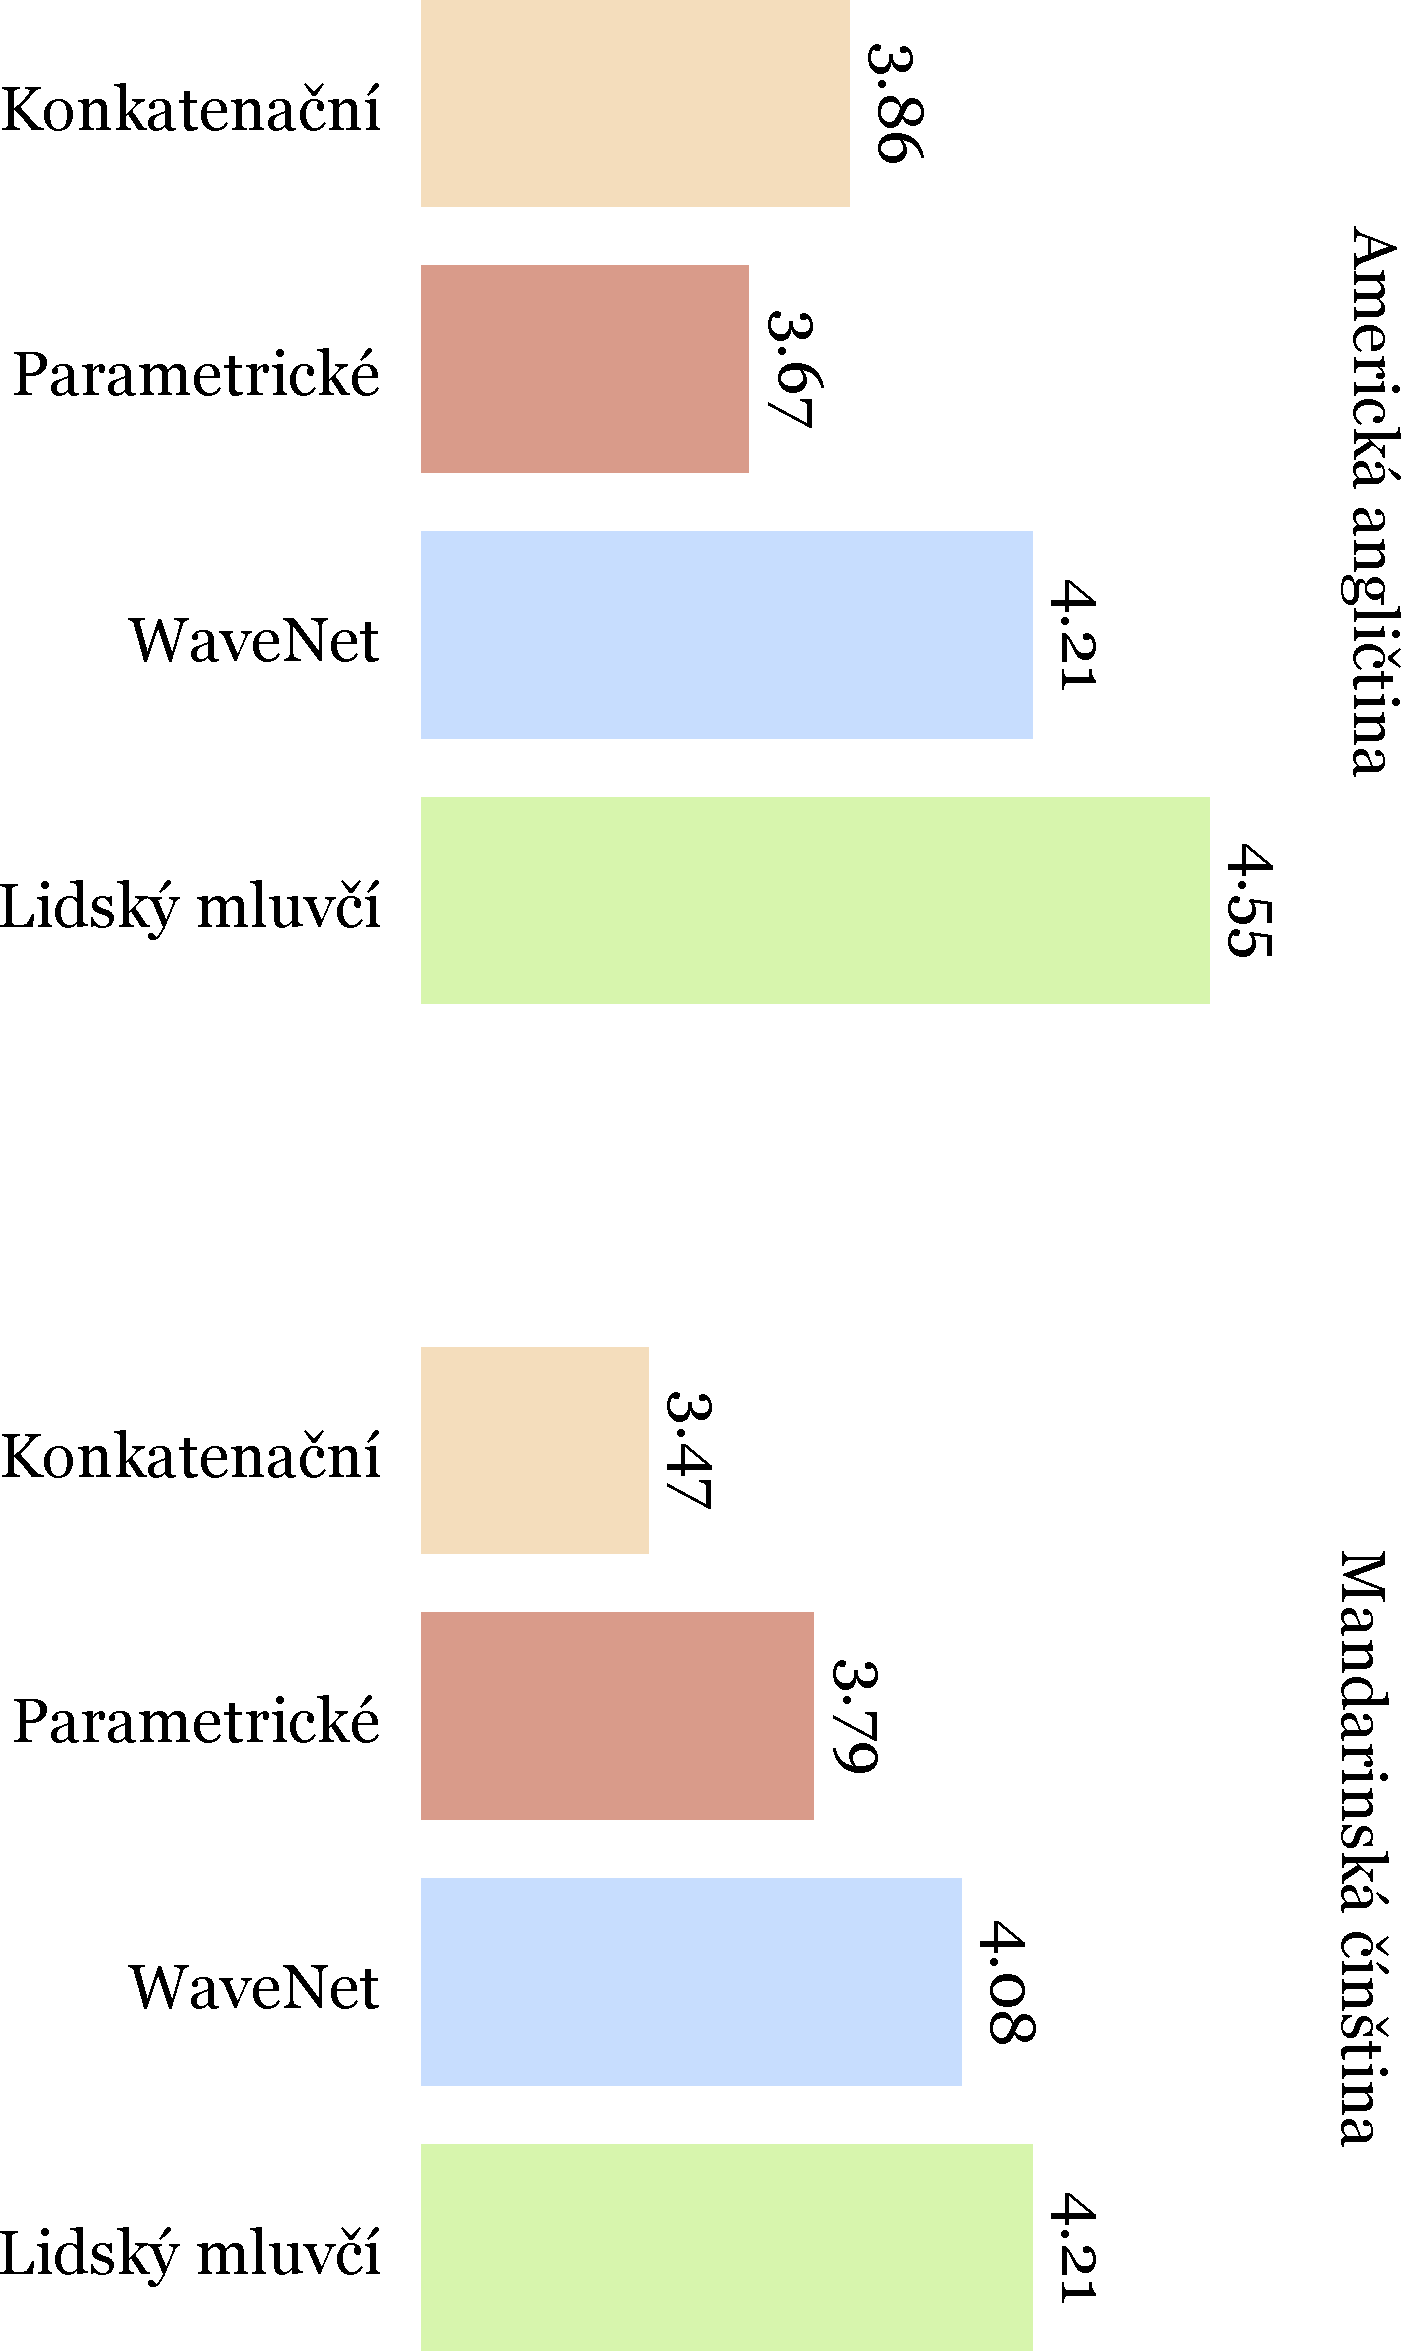
\includegraphics[angle=90, width=0.98\textwidth]{../img/wavenet-comparison.pdf}
    \caption{Porovnání průměrného hodnocení přirozenosti řeči na stupnici 1-5, převzato z dokumentace
        \citet[upraveno a přeloženo autorem]{google_tts}.}
    \label{img-wavenet}
\end{figure}